\hypertarget{a00006}{
\section{crf::crfPipe Class Reference}
\label{a00006}\index{crf::crfPipe@{crf::crfPipe}}
}
The \hyperlink{a00043}{crf} pipe inherits from the basic \hyperlink{a00045}{eqOsg} pipe, to add more features like event-adapting, scenegraph updates etc.  


{\tt \#include $<$crfPipe.h$>$}

Inherits \hyperlink{a00014}{eqOsg::Pipe}.

Collaboration diagram for crf::crfPipe:\nopagebreak
\begin{figure}[H]
\begin{center}
\leavevmode
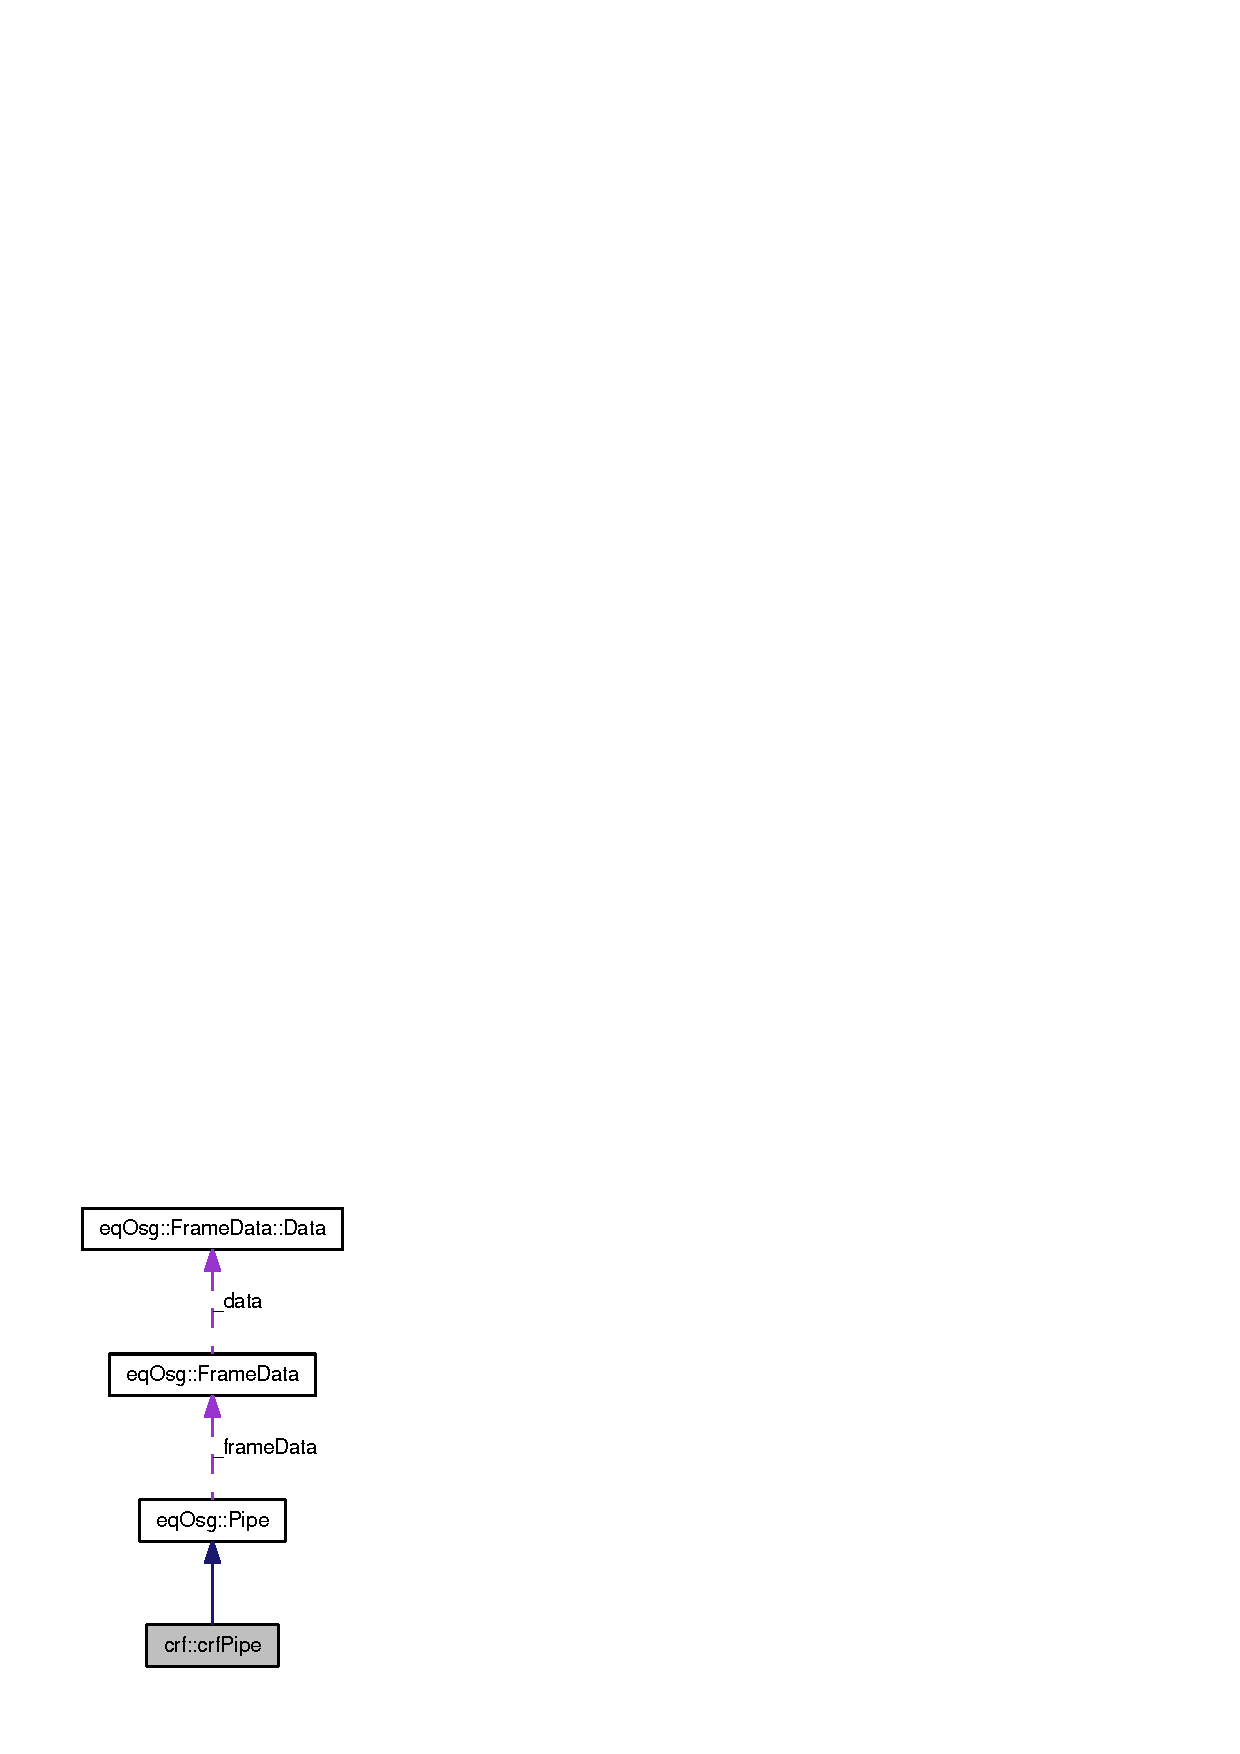
\includegraphics[width=168pt]{a00076}
\end{center}
\end{figure}
\subsection*{Public Member Functions}
\begin{CompactItemize}
\item 
\hyperlink{a00006_0b43238e38fb190f8a5e9a6148950ea0}{crfPipe} (eq::Node $\ast$parent)
\begin{CompactList}\small\item\em Creates a pipe with the empty viewer. \item\end{CompactList}\item 
\hyperlink{a00006_f5c46c7219b170979654b9e0defda4a7}{crfPipe} (eq::Node $\ast$parent, osg::ref\_\-ptr$<$ \hyperlink{a00009}{eqOsg::EqViewer} $>$ viewer)
\begin{CompactList}\small\item\em Creates a pipe with a given viewer. \item\end{CompactList}\item 
\hyperlink{a00006_d1215b24804515699867f0e718eb6985}{crfPipe} (eq::Node $\ast$parent, osg::ref\_\-ptr$<$ osg::Node $>$ sceneNode)
\begin{CompactList}\small\item\em Creates a pipe with a given osg scene node. \item\end{CompactList}\end{CompactItemize}
\subsection*{Protected Member Functions}
\begin{CompactItemize}
\item 
virtual void \hyperlink{a00006_2e551fe08841da2b7a1def541656d48c}{frameStart} (const uint32\_\-t frameID, const uint32\_\-t frameNumber)
\begin{CompactList}\small\item\em Starts the frame and calls converEqEventsToOsg(). \item\end{CompactList}\item 
virtual bool \hyperlink{a00006_fcf11863d5370a815bd7e1216cc0f2e6}{configInit} (const uint32\_\-t initID)
\begin{CompactList}\small\item\em Called when pipe gets initalised. \item\end{CompactList}\item 
virtual void \hyperlink{a00006_16ff3017a9a333b3c7dd21b2032567c4}{convertEqEventsToOsg} ()
\begin{CompactList}\small\item\em Take the eq-events out of the \_\-eventQueue in FrameData and pass it to the eqViewer. \item\end{CompactList}\item 
virtual void \hyperlink{a00006_44e473d6aa40bdb24ae85f1dfd1f973d}{createSceneGraph} ()
\begin{CompactList}\small\item\em Override this function to create the scene graph. \item\end{CompactList}\item 
virtual void \hyperlink{a00006_5288fedad120ffd32f3290b4c91065b7}{updateSceneGraph} ()
\begin{CompactList}\small\item\em Updates your scenegraph at the end of every frame. \item\end{CompactList}\item 
virtual void \hyperlink{a00006_44ac49a7ba2b74a56b00177009d09c93}{setUpViewer} ()
\begin{CompactList}\small\item\em This functions sets up the viewer. \item\end{CompactList}\item 
virtual void \hyperlink{a00006_61564c072f120d8898e57cb268118f9a}{convertKeyPressEvents} (eq::Event event)
\begin{CompactList}\small\item\em Convert the key press events. \item\end{CompactList}\item 
virtual void \hyperlink{a00006_9e4c676e2d880a7149d61c13f2e34f73}{convertKeyReleaseEvents} (eq::Event event)
\begin{CompactList}\small\item\em Convert the key release events. \item\end{CompactList}\item 
virtual void \hyperlink{a00006_bdce51a794891a4b0caa3f33ba6e7ab4}{convertMouseEvents} (eq::Event event)
\begin{CompactList}\small\item\em Converts the key press events. \item\end{CompactList}\item 
virtual bool \hyperlink{a00006_3f48f5f5a8a455342b111f26ca1402db}{configExit} ()
\begin{CompactList}\small\item\em Unref the viewer when closing. \item\end{CompactList}\end{CompactItemize}


\subsection{Detailed Description}
The \hyperlink{a00043}{crf} pipe inherits from the basic \hyperlink{a00045}{eqOsg} pipe, to add more features like event-adapting, scenegraph updates etc. 

Override this class' functions to create your own dynmaic and event depended scene graph. If you do so, don't forget to create your own \hyperlink{a00005}{crfNodeFactory} and pass it to \hyperlink{a00007}{crfStarter}, to force the CRF to use your objects. 

\subsection{Constructor \& Destructor Documentation}
\hypertarget{a00006_0b43238e38fb190f8a5e9a6148950ea0}{
\index{crf::crfPipe@{crf::crfPipe}!crfPipe@{crfPipe}}
\index{crfPipe@{crfPipe}!crf::crfPipe@{crf::crfPipe}}
\subsubsection[{crfPipe}]{\setlength{\rightskip}{0pt plus 5cm}crf::crfPipe::crfPipe (eq::Node $\ast$ {\em parent})\hspace{0.3cm}{\tt  \mbox{[}inline\mbox{]}}}}
\label{a00006_0b43238e38fb190f8a5e9a6148950ea0}


Creates a pipe with the empty viewer. 

Sets \_\-sceneGraphCreated to false! \begin{Desc}
\item[Parameters:]
\begin{description}
\item[{\em parent}]The pipe's Parent (a node). \end{description}
\end{Desc}
\begin{Desc}
\item[See also:]\hyperlink{a00014}{eqOsg::Pipe} \end{Desc}
\hypertarget{a00006_f5c46c7219b170979654b9e0defda4a7}{
\index{crf::crfPipe@{crf::crfPipe}!crfPipe@{crfPipe}}
\index{crfPipe@{crfPipe}!crf::crfPipe@{crf::crfPipe}}
\subsubsection[{crfPipe}]{\setlength{\rightskip}{0pt plus 5cm}crfPipe::crfPipe (eq::Node $\ast$ {\em parent}, \/  osg::ref\_\-ptr$<$ {\bf eqOsg::EqViewer} $>$ {\em viewer})}}
\label{a00006_f5c46c7219b170979654b9e0defda4a7}


Creates a pipe with a given viewer. 

\begin{Desc}
\item[See also:]\hyperlink{a00014}{eqOsg::Pipe} \end{Desc}
\begin{Desc}
\item[Parameters:]
\begin{description}
\item[{\em parent}]The pipe's parent. \item[{\em viewer}]The Pointer to a complete independent \hyperlink{a00009}{eqOsg::EqViewer}. \end{description}
\end{Desc}
\hypertarget{a00006_d1215b24804515699867f0e718eb6985}{
\index{crf::crfPipe@{crf::crfPipe}!crfPipe@{crfPipe}}
\index{crfPipe@{crfPipe}!crf::crfPipe@{crf::crfPipe}}
\subsubsection[{crfPipe}]{\setlength{\rightskip}{0pt plus 5cm}crfPipe::crfPipe (eq::Node $\ast$ {\em parent}, \/  osg::ref\_\-ptr$<$ osg::Node $>$ {\em sceneNode})}}
\label{a00006_d1215b24804515699867f0e718eb6985}


Creates a pipe with a given osg scene node. 

\begin{Desc}
\item[See also:]\hyperlink{a00014}{eqOsg::Pipe} \end{Desc}
\begin{Desc}
\item[Parameters:]
\begin{description}
\item[{\em parent}]The pipe's parent. \item[{\em sceneNode}]The scene node to display. This osg node is gonna be insereted as sceneData to the EqViewer. \end{description}
\end{Desc}


\subsection{Member Function Documentation}
\hypertarget{a00006_3f48f5f5a8a455342b111f26ca1402db}{
\index{crf::crfPipe@{crf::crfPipe}!configExit@{configExit}}
\index{configExit@{configExit}!crf::crfPipe@{crf::crfPipe}}
\subsubsection[{configExit}]{\setlength{\rightskip}{0pt plus 5cm}bool crfPipe::configExit ()\hspace{0.3cm}{\tt  \mbox{[}protected, virtual\mbox{]}}}}
\label{a00006_3f48f5f5a8a455342b111f26ca1402db}


Unref the viewer when closing. 

\begin{Desc}
\item[Returns:]True if everything worked fine. \end{Desc}
\begin{Desc}
\item[See also:]eqOsg::configExit \end{Desc}


Reimplemented from \hyperlink{a00014_2cb47387a7be185b1dc6d097dc4da38e}{eqOsg::Pipe}.\hypertarget{a00006_fcf11863d5370a815bd7e1216cc0f2e6}{
\index{crf::crfPipe@{crf::crfPipe}!configInit@{configInit}}
\index{configInit@{configInit}!crf::crfPipe@{crf::crfPipe}}
\subsubsection[{configInit}]{\setlength{\rightskip}{0pt plus 5cm}bool crfPipe::configInit (const uint32\_\-t {\em initID})\hspace{0.3cm}{\tt  \mbox{[}protected, virtual\mbox{]}}}}
\label{a00006_fcf11863d5370a815bd7e1216cc0f2e6}


Called when pipe gets initalised. 

CreateSceneGraph() is called here if \_\-sceneGraphCreated is still set to false. \begin{Desc}
\item[Returns:]True if everything worked fine. \end{Desc}
\begin{Desc}
\item[See also:]eqOsg::configInit \end{Desc}


Reimplemented from \hyperlink{a00014_d23bd6f7bb0f59f94fc0e279dbbb9d9a}{eqOsg::Pipe}.\hypertarget{a00006_16ff3017a9a333b3c7dd21b2032567c4}{
\index{crf::crfPipe@{crf::crfPipe}!convertEqEventsToOsg@{convertEqEventsToOsg}}
\index{convertEqEventsToOsg@{convertEqEventsToOsg}!crf::crfPipe@{crf::crfPipe}}
\subsubsection[{convertEqEventsToOsg}]{\setlength{\rightskip}{0pt plus 5cm}void crfPipe::convertEqEventsToOsg ()\hspace{0.3cm}{\tt  \mbox{[}protected, virtual\mbox{]}}}}
\label{a00006_16ff3017a9a333b3c7dd21b2032567c4}


Take the eq-events out of the \_\-eventQueue in FrameData and pass it to the eqViewer. 

Basic implementation, converts only basic keys yet.

This function can be OS depended, because eq does not report the same ascii codes for every windowing system! Actually all basic keys and some special keys are forewarded to the osg viewer. In Windows, the pushed ascii codes represent upper case letters. \hypertarget{a00006_61564c072f120d8898e57cb268118f9a}{
\index{crf::crfPipe@{crf::crfPipe}!convertKeyPressEvents@{convertKeyPressEvents}}
\index{convertKeyPressEvents@{convertKeyPressEvents}!crf::crfPipe@{crf::crfPipe}}
\subsubsection[{convertKeyPressEvents}]{\setlength{\rightskip}{0pt plus 5cm}void crfPipe::convertKeyPressEvents (eq::Event {\em event})\hspace{0.3cm}{\tt  \mbox{[}protected, virtual\mbox{]}}}}
\label{a00006_61564c072f120d8898e57cb268118f9a}


Convert the key press events. 

\begin{Desc}
\item[Parameters:]
\begin{description}
\item[{\em event}]The eq event to convert \end{description}
\end{Desc}
\hypertarget{a00006_9e4c676e2d880a7149d61c13f2e34f73}{
\index{crf::crfPipe@{crf::crfPipe}!convertKeyReleaseEvents@{convertKeyReleaseEvents}}
\index{convertKeyReleaseEvents@{convertKeyReleaseEvents}!crf::crfPipe@{crf::crfPipe}}
\subsubsection[{convertKeyReleaseEvents}]{\setlength{\rightskip}{0pt plus 5cm}void crfPipe::convertKeyReleaseEvents (eq::Event {\em event})\hspace{0.3cm}{\tt  \mbox{[}protected, virtual\mbox{]}}}}
\label{a00006_9e4c676e2d880a7149d61c13f2e34f73}


Convert the key release events. 

convert the key release events

\begin{Desc}
\item[Parameters:]
\begin{description}
\item[{\em event}]The eq event to convert \end{description}
\end{Desc}
\hypertarget{a00006_bdce51a794891a4b0caa3f33ba6e7ab4}{
\index{crf::crfPipe@{crf::crfPipe}!convertMouseEvents@{convertMouseEvents}}
\index{convertMouseEvents@{convertMouseEvents}!crf::crfPipe@{crf::crfPipe}}
\subsubsection[{convertMouseEvents}]{\setlength{\rightskip}{0pt plus 5cm}void crfPipe::convertMouseEvents (eq::Event {\em event})\hspace{0.3cm}{\tt  \mbox{[}protected, virtual\mbox{]}}}}
\label{a00006_bdce51a794891a4b0caa3f33ba6e7ab4}


Converts the key press events. 

convert the mouse events

\begin{Desc}
\item[Parameters:]
\begin{description}
\item[{\em event}]The eq event to convert \end{description}
\end{Desc}
\hypertarget{a00006_44e473d6aa40bdb24ae85f1dfd1f973d}{
\index{crf::crfPipe@{crf::crfPipe}!createSceneGraph@{createSceneGraph}}
\index{createSceneGraph@{createSceneGraph}!crf::crfPipe@{crf::crfPipe}}
\subsubsection[{createSceneGraph}]{\setlength{\rightskip}{0pt plus 5cm}void crfPipe::createSceneGraph ()\hspace{0.3cm}{\tt  \mbox{[}protected, virtual\mbox{]}}}}
\label{a00006_44e473d6aa40bdb24ae85f1dfd1f973d}


Override this function to create the scene graph. 

Pass the root node of the scene graph to the \_\-viewer member, add OSG eventhandlers if desired etc... \hypertarget{a00006_2e551fe08841da2b7a1def541656d48c}{
\index{crf::crfPipe@{crf::crfPipe}!frameStart@{frameStart}}
\index{frameStart@{frameStart}!crf::crfPipe@{crf::crfPipe}}
\subsubsection[{frameStart}]{\setlength{\rightskip}{0pt plus 5cm}void crfPipe::frameStart (const uint32\_\-t {\em frameID}, \/  const uint32\_\-t {\em frameNumber})\hspace{0.3cm}{\tt  \mbox{[}protected, virtual\mbox{]}}}}
\label{a00006_2e551fe08841da2b7a1def541656d48c}


Starts the frame and calls converEqEventsToOsg(). 

\begin{Desc}
\item[See also:]eqOsg::Pipe::framestart \end{Desc}


Reimplemented from \hyperlink{a00014_6be431b1b9fe04da31596ea8b870dfde}{eqOsg::Pipe}.\hypertarget{a00006_44ac49a7ba2b74a56b00177009d09c93}{
\index{crf::crfPipe@{crf::crfPipe}!setUpViewer@{setUpViewer}}
\index{setUpViewer@{setUpViewer}!crf::crfPipe@{crf::crfPipe}}
\subsubsection[{setUpViewer}]{\setlength{\rightskip}{0pt plus 5cm}void crfPipe::setUpViewer ()\hspace{0.3cm}{\tt  \mbox{[}protected, virtual\mbox{]}}}}
\label{a00006_44ac49a7ba2b74a56b00177009d09c93}


This functions sets up the viewer. 

Currently an OSG statshandler is added and listen to the F2 keystroke. Override this function to specify your viewer. \hypertarget{a00006_5288fedad120ffd32f3290b4c91065b7}{
\index{crf::crfPipe@{crf::crfPipe}!updateSceneGraph@{updateSceneGraph}}
\index{updateSceneGraph@{updateSceneGraph}!crf::crfPipe@{crf::crfPipe}}
\subsubsection[{updateSceneGraph}]{\setlength{\rightskip}{0pt plus 5cm}virtual void crf::crfPipe::updateSceneGraph ()\hspace{0.3cm}{\tt  \mbox{[}inline, protected, virtual\mbox{]}}}}
\label{a00006_5288fedad120ffd32f3290b4c91065b7}


Updates your scenegraph at the end of every frame. 

Override this function to create your own frame/time related animations. Basic Implementation: empty! 

The documentation for this class was generated from the following files:\begin{CompactItemize}
\item 
E:/schule/Thesis/Repo/trunk/crf/src/crfPipe.h\item 
E:/schule/Thesis/Repo/trunk/crf/src/crfPipe.cpp\end{CompactItemize}
